% Preamble templated from Mihir-Divyansh/Course-Setup
%iffalse
\let\negmedspace\undefined
\let\negthickspace\undefined
\documentclass[journal,12pt,onecolumn]{IEEEtran}
\usepackage{cite}
\usepackage{amsmath,amssymb,amsfonts,amsthm}
\usepackage{algorithmic}
\usepackage{graphicx}
\usepackage{textcomp}
\usepackage{xcolor}
\usepackage{txfonts}
\usepackage{listings}
\usepackage{enumitem}
\usepackage{mathtools}
\usepackage{gensymb}
\usepackage{comment}
\usepackage[breaklinks=true]{hyperref}
\usepackage{tkz-euclide}
\usepackage{listings}
\usepackage{gvv}
%\def\inputGnumericTable{}
\usepackage[latin1]{inputenc}
\usepackage{color}
\usepackage{array}
\usepackage{longtable}
\usepackage{calc}
\usepackage{multirow}
\usepackage{hhline}
\usepackage{ifthen}
\usepackage{lscape}
\usepackage{tabularx}
\usepackage{array}
\usepackage{float}
\usepackage{caption}
\usepackage{multicol}

\newtheorem{theorem}{Theorem}[section]
\newtheorem{problem}{Problem}
\newtheorem{proposition}{Proposition}[section]
\newtheorem{lemma}{Lemma}[section]
\newtheorem{corollary}[theorem]{Corollary}
\newtheorem{example}{Example}[section]
\newtheorem{definition}[problem]{Definition}
\newcommand{\BEQA}{\begin{eqnarray}}
\newcommand{\EEQA}{\end{eqnarray}}
%\newcommand{\define}{\stackrel{\triangle}{=}}
\theoremstyle{remark}
%\newtheorem{rem}{Remark}

% Marks the beginning of the document
\begin{document}
\bibliographystyle{IEEEtran}
\vspace{3cm}

\title{Assignment 6: 4.3.45}
\author{EE25BTECH11055 - Subhodeep Chakraborty}
\maketitle
\hrulefill
\bigskip

\renewcommand{\thefigure}{\theenumi}
\renewcommand{\thetable}{\theenumi}

\textbf{Question:}\par
Find the coordinates of the point where the line through \brak{5, 1, 6} and \brak{3, 4, 1} crosses the $YX$-plane.
\par
\textbf{Solution:}\par

Given:
\begin{align}
 \vec{A} = \myvec{5\\1\\6} \\
 \vec{B} = \myvec{3\\4\\1}
\end{align}

We know,
\begin{align}
 \vec{x} &= \vec{h} +k\vec{m} \\
 &= \vec{A} + k\brak{\vec{B-A}} \\
 \vec{e_3}^\top\vec{x} &= 0
\end{align}
Thus
\begin{align}
 \vec{e_3}^\top\vec{A} + &k\vec{e_3}^\top\brak{\vec{B-A}} = 0 \\
 k &= \frac{\vec{e_3}^\top\vec{A}}{\vec{e_3}^\top\vec{A}-\vec{e_3}^\top\vec{B}} \\
 \vec{x} &= \vec{A} + \frac{\vec{e_3}^\top\vec{A}}{\vec{e_3}^\top\vec{A}-\vec{e_3}^\top\vec{B}}\brak{\vec{B-A}}
\end{align}
Solving
\begin{align}
\vec{e_3}^\top\vec{A} &= 6 \\
\vec{e_3}^\top\vec{B} &= 1 \\
 \vec{x} &= \myvec{5-2\times\dfrac{6}{5} \\ 1+3\times\dfrac{6}{5} \\ 6-5\times\dfrac{6}{5}} \\
  \vec{x} &= \myvec{13/5 \\ 23/5 \\ 0}
\end{align}
\begin{figure}[H]
    \centering
    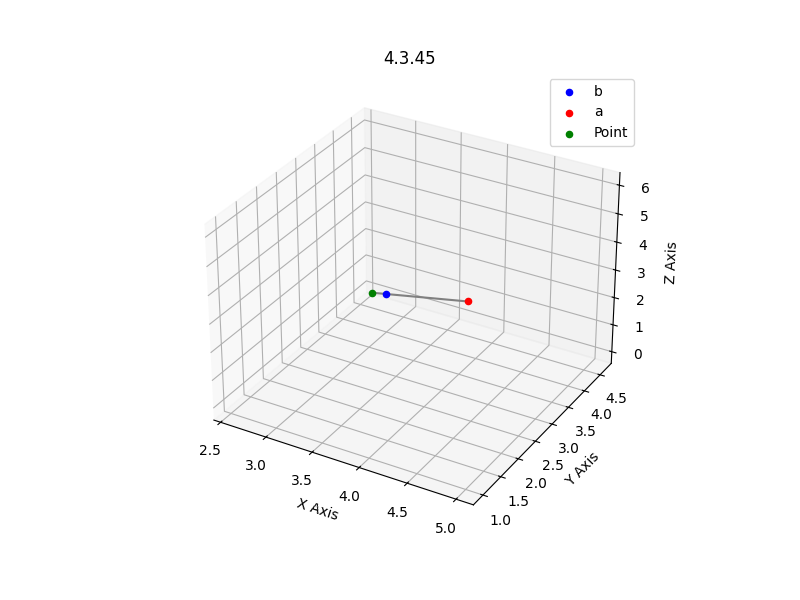
\includegraphics{figs/plot.png}
    \caption*{}
    \label{fig:plot}
\end{figure}
\end{document}
